\chapter{Applications and Use Cases}
\label{chapter:applications}
\epiquote{If your only tool is a hammer then every problem looks like a nail.}{Abraham Maslow, 1966}

An aspect that has always fascinated me about computer science and information technology is, that it has applications in every conceivable domain. It is this combination of purely technological aspects -- the computational part -- and the domain knowledge, that make this field challenging as well as interesting. Digital transformation -- the act of improving businesses and processing using digital technology \cite{Vial:2019Understanding} -- has been a driving force behind economic activity over the past decade, and while many non-technological factors define digital transformation, optimisation through the application of dispruptive technologiies remains the main incentive behind it.

It is therefore, that we do not want to detach the work presented in this Thesis from its concrete applications and instead aim to motivate it based on real-world scenarios. We do so, by introducing three use-cases, where we believe that a multimedia database system fulfills an important function. From these use-cases, we derive a series of requirements that motivate the importance of such a dedicated, general-purpose multimedia database.

\section{Use case 1: Multimedia Retrieval Applications}
\label{section:application_retrieval}

Multimedia retrieval in a broader sense describes the act of finding items of interest in large, multimedia collections, wherein ``multimedia'' can refer to any type of modality, such as text, images, videos or audio and any combination thereof. Consequently, a multimedia retrieval system must be able to have a user express their \emph{information need} as a \emph{query} that the system can then use to (ideally) produce the item(s) of interest as a \emph{result}. The process is visualized in \Cref{figure:mr-ideal} and a formal problem definition will be provided in \Cref{chapter:theory_multimedia_analysis_and_retrieval}.

\begin{figure}[tb]
    \centering
    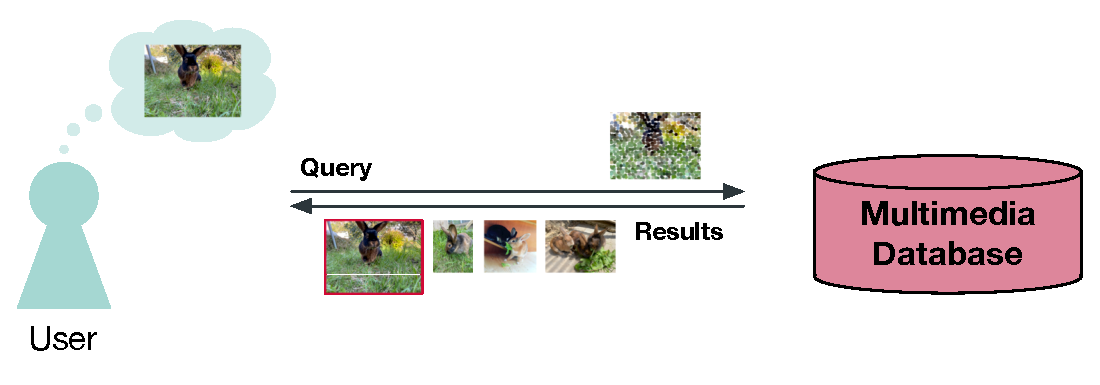
\includegraphics[width=\textwidth]{figures/mr-ideal.eps}
    \caption{The idealised multimedia retrieval problem: A user expresses an information need as a query and the multimedia retrieval system returns matching items from a collection as a resultset, ideally including the desired item.}
    \label{figure:mr-ideal}
\end{figure}

There are umpteenth potential applications of the multimedia retrieval problem, but to name a few, one could consider collections produced by radio or TV stations that must be made searchable \cite{Watanabe:1998Multimedia}, collections of cultural heritage data as maintained by museums, archives and archaeology departments \cite{Tsai:2007Review} or medical image collections containing X-rays or \acrshort{mri} images \cite{Mueller:2004Review}.

What makes multimedia retrieval a challenging problem is the inherently unstructured nature of the data that we deal with, by which we mean that the raw, (digital) information may not directly reflect the content of the item as we -- as human consumers -- might perceive or describe it. Let us take, for example, the image we were looking for in \Cref{figure:mr-ideal}. If our task were to describe that image so that we can retrieve it from a large database\footnote{This example is purposely neglecting the influence of memory, from which a user might reconstruct the image, which makes the problem even more challenging.}, we might use terms like ``rabbit'' or ``grass''. We might assume, judging from the image, that the scene is taking place in a ``garden'' and maybe we notice that the rabbit is currently ``munching'' on a ``leaf'' or ``strain of grass''. We might even know the rabbit's breed or name, if we were to be its owner.

All of this information is formed based on a series of steps ranging from perception, over interpretation to cognition as illustrated in \Cref{figure:knowledge_formation} and each of these steps is accompanied by a loss or distortion of information \cite{Javanmardi:2021Exploring,Rossetto:2018thesis}, which makes this process highly subjective, giving rise to a series of ``gaps'' that influence the outcome. Most importantly, however, all of the aforementioned descriptions are not explicitly contained in the raw image data, which is merely an array of colour values that constitutes the image and does neither come pre-labeled nor pre-described.

\begin{figure}[tb]
    \centering
    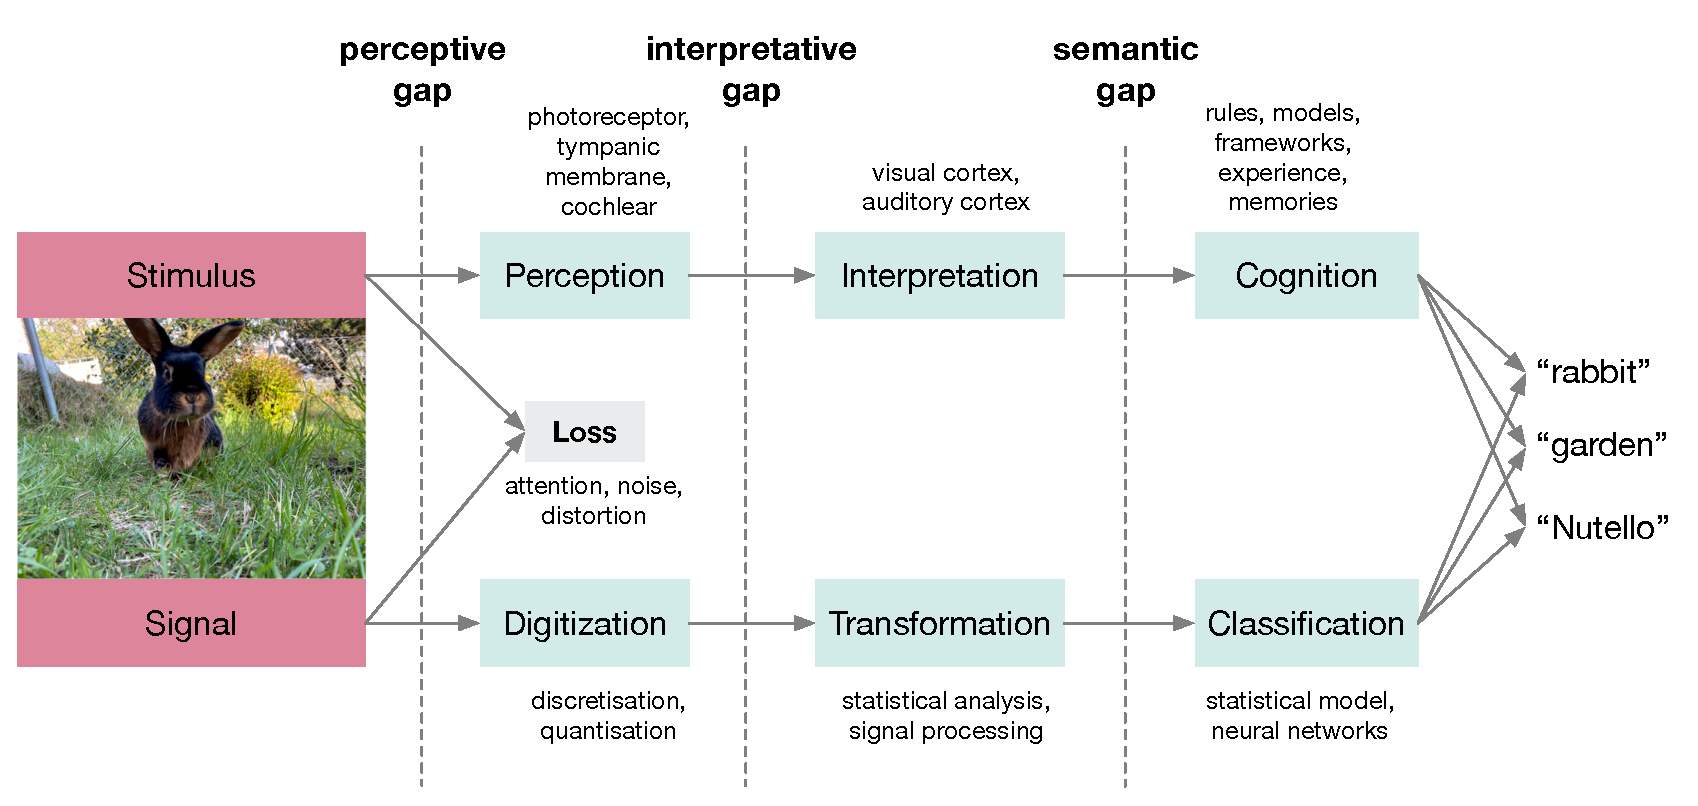
\includegraphics[width=\textwidth]{figures/gaps.eps}
    \caption{A simplified model of knowledge formation in humans (adapted from \cite{Javanmardi:2021Exploring}) and machines.}
    \label{figure:knowledge_formation}
\end{figure}

This impedance mismatch between the content being stored and the information required to find it, is the main challenge that unstructured data brings with it, as opposed to structured data where retrievable units of information are directly contained in the data itself. Bridging these gaps between the information available and the information we might use to actually search for an item of interest is therefore one of the major obstacles to overcome in multimedia retrieval. Over the years, different solutions have been developed:

\begin{description}
    \item[Manual Labeling] The obvious solution is to manually embed the aforementioned labels and descriptions into the multimedia item so that we can use this information to find it at a later point in time. While as of today, this approach is still widely used, it comes with two important disadvantages. Obviously, it remains a subjective task, because as we have argued, the process of forming these labels may yield different results depending on who is assigning them (due to the perceptive, interpretative and semantic gap). Most importantly, though, the task of manual label assignment is laborious and unable to scale with the ever increasing velocity at which multimedia data is produced.
    \item[Automatic Labeling] Recent advantages in machine learning has provided us with the ability to automatically label different types of multimedia through classification. So instead of describing the content ourselves, we can leave this to pre-trained models that have (at a very high level) a similar mode of operation as a human consumer, as is illustrated in \Cref{figure:knowledge_formation}. While this solves the problem of scalability, it remains a subjective task since training the models is also subject to the aforementioned gaps. Furthermore, there may be discrepancies between the (mental) model used for classification and the one employed during query formulation, which typically take place at different points in time and are carried out by different people.
    \item[Content-Based Search] The last approach and the one that ``classical'' multimedia retrieval has concerned itself with for years is that of \emph{content-based search}. Instead of using the higher-level concepts, content-based search works with intermediate representations called \emph{descriptors} that are derived from the data using signal processing or statistical analysis. These descriptors -- which are often real-valued vectors -- can then be used to establish a notion of \emph{similarity} between items in a collection and a query. This is called  the \emph{vector space model} for similarity search. In this context, the term query may refer to more than simply textual input. Given the example in \Cref{figure:mr-ideal}, we could use another image of a rabbit as a query (Query-by-Example, \cite{Kelly:1995Query}) or try to create a sketch to find the item we're interested in (Query-by-Sketch, \cite{Sciascio:1999Content}).
\end{description}

Decades of research and practice have shown that while individual methods falling into any of the three categories may yield acceptable or even exceptional results, there is clear indication that ultimately, a combination of the three is the most powerful solution, especially if the exact type of information need is not known in advance \todo{Find source}. Furthermore, we know from research and practice, that instead of the simple ``issue a query, get a result'' scheme illustrated in \Cref{figure:mr-ideal}, actual multimedia retrieval problems -- which we will henceforth refer to as interactive multimedia retrieval -- require a constant back and forth between system and user that include not only querying but also exploration, browsing, examination of items and query refinement \cite{Lokovc:2019Interactive,Gurrin:2019Invited}. This is something being explicitly tested at interactive retrieval competitions such as \acrfull{vbs} \cite{Schoeffmann:2019Video} or \acrfull{lsc} \cite{Gurrin:2021Introduction}. This interactive multimedia retrieval problem is illustrated in \Cref{figure:mr-actual} and we argue, that it poses very similar requirements to data management as a multimedia analytics \cite{Chinchor:2010Multimedia} workload would. The two aspects have important implications for data management systems: 

\begin{figure}[tb]
    \centering
    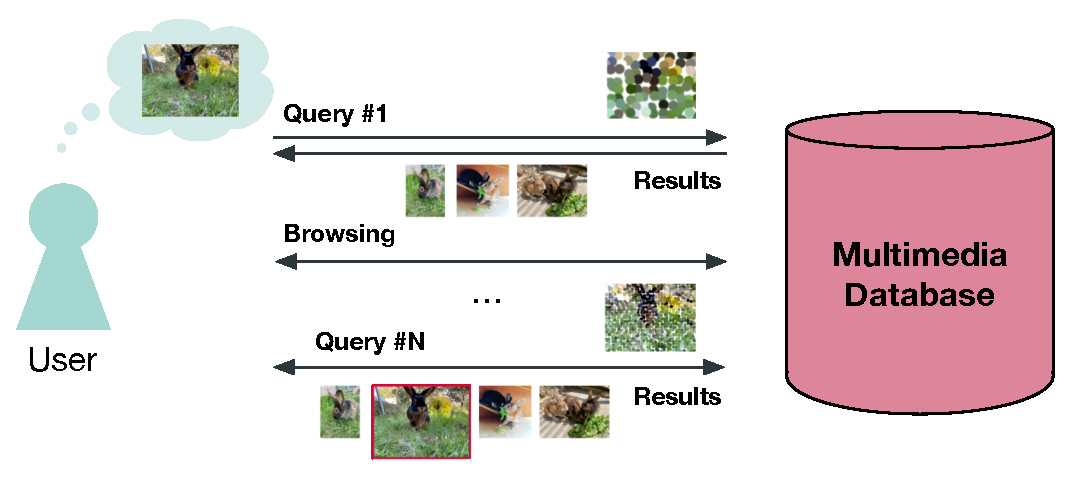
\includegraphics[width=\textwidth]{figures/mr-actual.eps}
    \caption{The interactive multimedia retrieval problem: A continuous back and forth between system and user involving different types of workload as the user tries to find the item of interest through query (re-)formulation, browsing and examination.}
    \label{figure:mr-actual}
\end{figure}
 
Firstly, we have to consider different data models when dealing with information from the aforementioned categories. While searching for labels and textual descriptions at scale can be achieved by the well-established \emph{Boolean retrieval} model, we require the completely different vector space retrieval model when dealing with descriptors derived from multimedia data and, ideally, we should have the ability to combine the two in unified queries, as e.g., proposed in the ``multi-stage queries'' presented in \cite{Heller:2020Multi}. This is a problem that has been acknowledged by other authors before \cite{Jonson:2016}  and that has been partially addressed, for example, by \cite{Giangreco:2018thesis,Giangreco:2016adam,Wang2021:Milvus}. However, all these approaches are limited in how such a combination is possible.

Secondly, any database management system supporting interactive multimedia retrieval workloads, must support different types of queries and it must be able to satisfy them in a reasonable amount of time, so that the user in the loop must not wait for results too long. This is especially important in timeboxed settings, as for example, evaluation campaigns such as \acrshort{vbs} or \acrshort{lsc}.

A third aspect, which cannot be derived directly from what has been described thus far, is the staticity of the data itself. We often implicitly assume that data collections remain static while they are being queried but it must be emphasized that this is very likely not to be true for a majority of data collections, which are continuously being worked on by users. 

All these requirements are very well summarised by Smeulders et al., who state that \emph{``The interacting user brings about many new challenges for the response time of the system. Content-based image retrieval is only scalable to large data sets when the database is able to anticipate what interactive queries will be made. A frequent assumption is that the image set, the features, and the similarity function are known in advance. In a truly interactive session, the assumptions are no longer valid.''} \cite{Smeulders:2000Content}

\section{Use case 2: Analysis of Social Media Streams}
\label{section:application_online_analysis}

Social media platforms such as Twitter\footnote{See https://www.twitter.com}, Facebook\footnote{See https://www.facebook.com}, Instagram\footnote{See https://www.instagram.com} and TikTok\footnote{See https://www.tiktok.com} have gained enormous traction over that past few decades. Current estimates suggest, that there are roughly $4.66$ billion active Internet users worldwide, of which $4.2$ billion can be considered active social media users\footnote{Source: Statista.com, ``Social media usage worldwide'', January 2021}. Facebook alone contributed to $144$ thousand uploaded images per minute in 2020. And many more of these  platforms, such as Instagram or Twitter, serve millions of users with self-made content involving text, images, videos or a combination thereof.

This brave new world of interaction and interconnection on different platforms, which are the sole source of information for a lot of people, has brought about new challenges in need of solutions. Probably the most important challenge is known under the umbrella term ``fake news'' \cite{Lazer:2018Science}, by which we mean information that is disguised as authentic news but contains fabricated, misleading or even wrong information. The term became highly polarised in the 2016 U.S. elections \cite{Quandt:2019Fake} where orchestrated campaigns on social media where used and may have tipped the scales in favour of the winning party. Ever since, political actors have used the term to invalidate the other side's arguments.

While the problem of fake news can arguably not be solved by merely technical means, the issue has brought about many different research questions in the realm of social media. One focus lies on the direct detection of misinformation on different channels \cite{Zhou:2020Survey} by different means such as content, propagation patterns or sources. Others try to tackle the detection of bots \cite{Cresci:2020Decade}, user-accounts that are not backed by real humans and that are often used to create or spread misinformation. And then there is the topic of sentiment analysis \cite{Yue:2019Survey}, which can yield important clues about how (fake-) news stories are received by their consumers.

While many of the aforementioned problems mainly deal with textual information, multimedia obviously plays an important role as well. Instagram and TikTok, for example, focus solely on the sharing of images and videos respectively. And a very recent and preliminary analysis suggests \cite{Ciuriak:2022Role}, that the sharing of images and videos plays an important role in the international covering of Russia's war on Ukraine. Potential problems in need of solution could, for example, be the automatic detection of image forgeries \cite{Farid:2009Image}.

If we examine what a fictious and generalised pipleine for social media analysis and analytics would look like, we might arrive at something as illustrated in \Cref{figure:social-media} (see, for example, \cite{Cui:2019Defend,Yang:2019XFake,Bagade:2020Kauwa}). The many different channels in existence, require for a broad range of tools that deal with data collection using crawlers or APIs provided by the respective source. Since all these potential sources are likely to use very different types of data models, some sort of integration into a common framework is very likely. This step may also be accompanied by data enrichtment using external services or data existing in the system's own collection. This is then followed by what we call analysis, which may include a wide range of machine learning and data analysis techniques that may or may not rely on existing data. A common theme for this step is that, similarily to multimedia retrieval, it probably involves generation and storage of formal descriptors of the multimedia content. Therefore, the entire pipeline is very likely to be backed by some type of persistent data store (the multimedia database), which can store labels, descriptors and metadata and which allows queries by both the analysis and the analytics components built on top of it -- both producing new data as well.

\begin{figure}[tb]
    \centering
    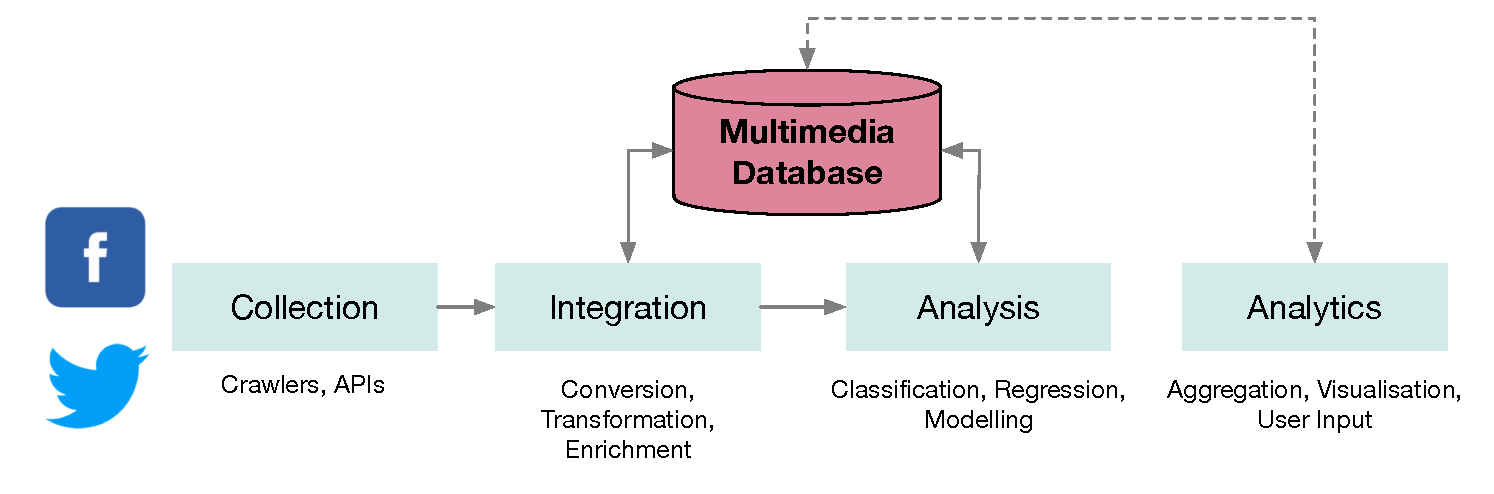
\includegraphics[width=0.90\textwidth]{figures/social-media-architecture.eps}
    \caption{A generalised architecture of a fictious social media analysis and analytics platform.}
    \label{figure:social-media}
\end{figure}

From the described architecture and the general flow of information, we can, again, derive certain needs with respect to the underlying database: Firstly, this database must be able to deal with changing, non-static data, since the various sources will potentially generate a steady and  continuous flow of information. APIs, such as Twitter's Firehose, are capable of producing data streams of hundreds of tweets per second \todo{Source?}.

Secondly, and similarily to the multimedia retrieval problem, we will deal with structured (e.g., technical metadata), semi-structured and unstructured information and all of this information needs to be stored somehow. Therefore, the data model employed by the multimedia database must be able to accept that data. 

And finally, with social media being a very classical field for applying multimedia analytics techniques \cite{Pouyanfar:2018,Jonson:2016}, the various tools that could be built upon the multimedia database will probably rely on a wide range of different query workloads, which the database should be able to support.

\section{Use case 3: Magnetic Resonance Fingerprinting (MRF)}
\label{section:application_mrf}

Multimedia retrieval for medical applications has been an important area of research for many decades now \cite{Mueller:2017Retrieval,Mueller:2004Review} and many of the arguments that we have made in \Cref{section:application_retrieval} can be repeated for this specialised sub-domain.

However, in this section, we want to focus on a very specific application, in which we do not consider media in the classical sense but in a broader sense of raw signals stemming from a \acrfull{mri} device.

\acrshort{mri} is a non-invasive, non-ionizing imaging technique that has gained huge importance in various fields of modern medicine. \acrshort{mri} is enabled by \acrfull{nmr}, which was first described by Purcell and Bloch in 1946 \cite{Bloch:1946Nuclear,Purcell:1946Resonance}. In simple terms, an \acrshort{mri}-machine operates by applying a very strong, external, magnetic field -- often referred to as $B_0$ -- which forces the protons in the matter to align to it. That field is disrupted by applying a second, radio-frequency pulse that interferes with the proton's alignment. When this pulse is switched of, the protons will re-align with $B_0$ over time in what is called relaxation. This process is characterized by the relaxation times $T_1$ and $T_2$, which are specific to a type of material and tissue, and accompanied by a short-term burst of energy that can be detected by the \acrshort{mri}-machine and which gives rise to the detected signal.

This technique has the ability to generate fine-grained contrasts in different types of soft tissue. However, it comes with two critical disadvantages: Firstly, there is an inherently long acquisition time that can range anything from several minutes to over an hour per scan, especially when one tries to achieve quantification of magnetic properties of soft tissue. Secondly, and due to this lack of fast, quantitative tools, MRI images have become mostly qualitative in nature. Anatomical areas are often referred to as either ``hyperintense'' or ``hypointense'' with respect to their immediate surrounding, but the difference between such areas or even the absolute values themselves cannot be measured directly.

\acrfull{mrf} is a technique \cite{Ma:2013Magnetic} that proposes a solution to this problem. In summary, \acrshort{mrf} is based on the assumption that different types of tissue produce a distinct signal evolution -- called \emph{fingerprint} -- when exposed a specific acquisition scheme. Simply put, it means that during data acquisition, measurements take place under varying, external magnetic fields and RF-pulses and signals are recorded for the different configurations resulting in the fingerprint. That fingerprint can then be matched against a database (called dictionary) of pre-calculated, discretised fingerprints that have been simulated using \emph{Bloch}'s theorem of magnetic resonance \cite{Bloch:1946Nuclear}. Through that matching step, values for $B_0$, $T_1$ and $T_2$ can be obtained. The overall process is described very well in \cite{Bipin:2019Magnetic} and illustrated in \Cref{figure:mrf}.

\begin{figure}[tb]
    \centering
    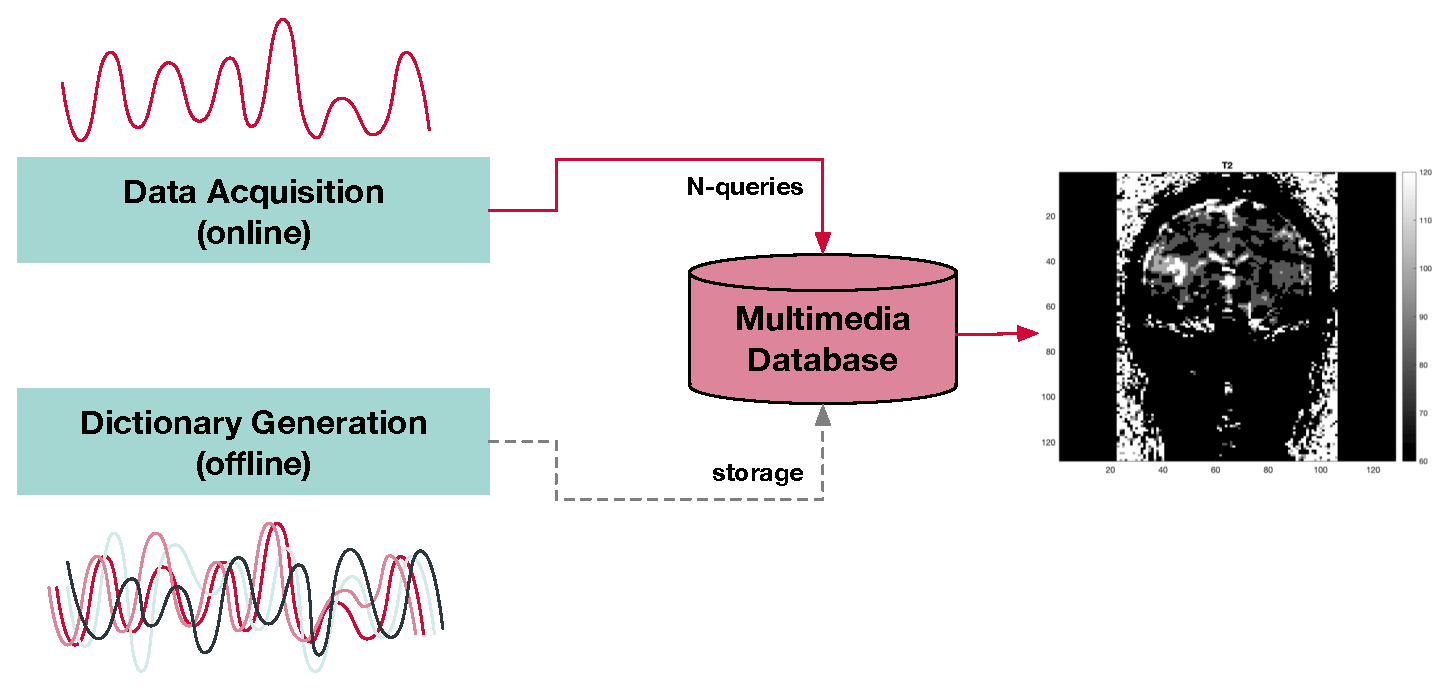
\includegraphics[width=\textwidth]{figures/mrf.eps}
    \caption{Simplified block diagram of a \acrshort{mrf} system: The data dictionray is generated and stored in an offline phase. During data acquisition, multiple signal vector are obtained and matched against the database to form the image (adapted from \cite{Bipin:2019Magnetic}, reconstruction of brain scan kindly provided by Manuel Hürbin).}
    \label{figure:mrf}
\end{figure}

While many techniques have been proposed to realise the matching step, at its core it involves performing \acrfull{mips} of complex singal vectors $v \in \symcomplex$ against a database of complex signal vectors. Since matching vectors against large databases of vectors is something done quite frequently in multimedia retrieval, it can be seen as a very similar problem. 

However, when compared to multimedia retrieval, there are a few important exceptions: 

\begin{itemize}
    \item The vectors compared in \acrshort{mrf} are complex and not real-valued.
    \item The inner product obtained is maximized and not minimized.
    \item Since the dictionary is a discretization of a continuous, simulated signal, the data is very dense as opposed to often sparse data in multimedia retrieval.
\end{itemize}

\section{Deriving Requirements}
From the use cases presented in Sections \ref{section:application_retrieval}, \ref{section:application_online_analysis} and \ref{section:application_mrf} we can see the need for a dedicated \emph{multimedia database} that can store and manage the the different types of data produced by the described examples and that can execute the different types of workloads. In this section, we will list a series of concrete requirements posed to such a \emph{multimedia database}.

\begin{requirement}{Requirement Hello World}
    This is a requirement.
\end{requirement}